% !TEX root = ./../paper.tex

\section{Results}
\label{sec:results}

\subsection{Language}
\label{sec:results:language}

\sculpt as a programming language is a functioning language capable of writing any program.

As a first example and introduction to the language itself, we have implemented a simple program that calculates the Fibonacci sequence in \sculpt.

The language uses FILO (First In Last Out) stacks as its only data structure to store and manipulate data. Each stack is represented by a different shape other than the reserved shapes used by the instructions, and they are initialized on first call.
Stacks can hold an arbitrarily large amount of rational numbers.
Stacks allow the pop, push, move and duplicate operations.
Numbers are defined by their literal counterparts, and the language supports basic arithmetic.
Arithmetic operations are the only operations available in \sculpt.
Availabre operations are addition, subtraction, multiplication, comparison, modulo and division.
These are performed in two ways:

\begin{itemize}
    \item \textbf{As unary operator}: The first two elements of the stack given by parameter are popped and operated and pushing the result back into the stack.
    \item \textbf{As binary operator}: The first element of the stack given by parameter is popped and the second parameter, a number, are operated with the result of the first operation. The result is pushed back into the stack.
\end{itemize}

\sculpt allows for flow control through the use of loops, conditional blocks and jump blocks.
Loops are physically represented by a literal loop of connected blocks or a single block jump.
The jump block is a special block that allows for the execution to continue at any point by moving the execution pointer from the current block to another with the offset given by parameter.
Conditional statements are represented by a question block using a stack value as a parameter. Positive values are considered true and evaluate the following block, and negative values are considered false and do not evaluate the affected block, but rather skips the next instruction.


\sculpt is based on the physical blocks. Blocks as three-dimensional objects are unwieldy to be described in text.
Therefore, we have made several valid notations for \sculpt programs.
Every block is represented as a square with the shape of each block inside the square. 
The connections between blocks are represented by arrows between the squares.

\begin{figure}
    \centering
    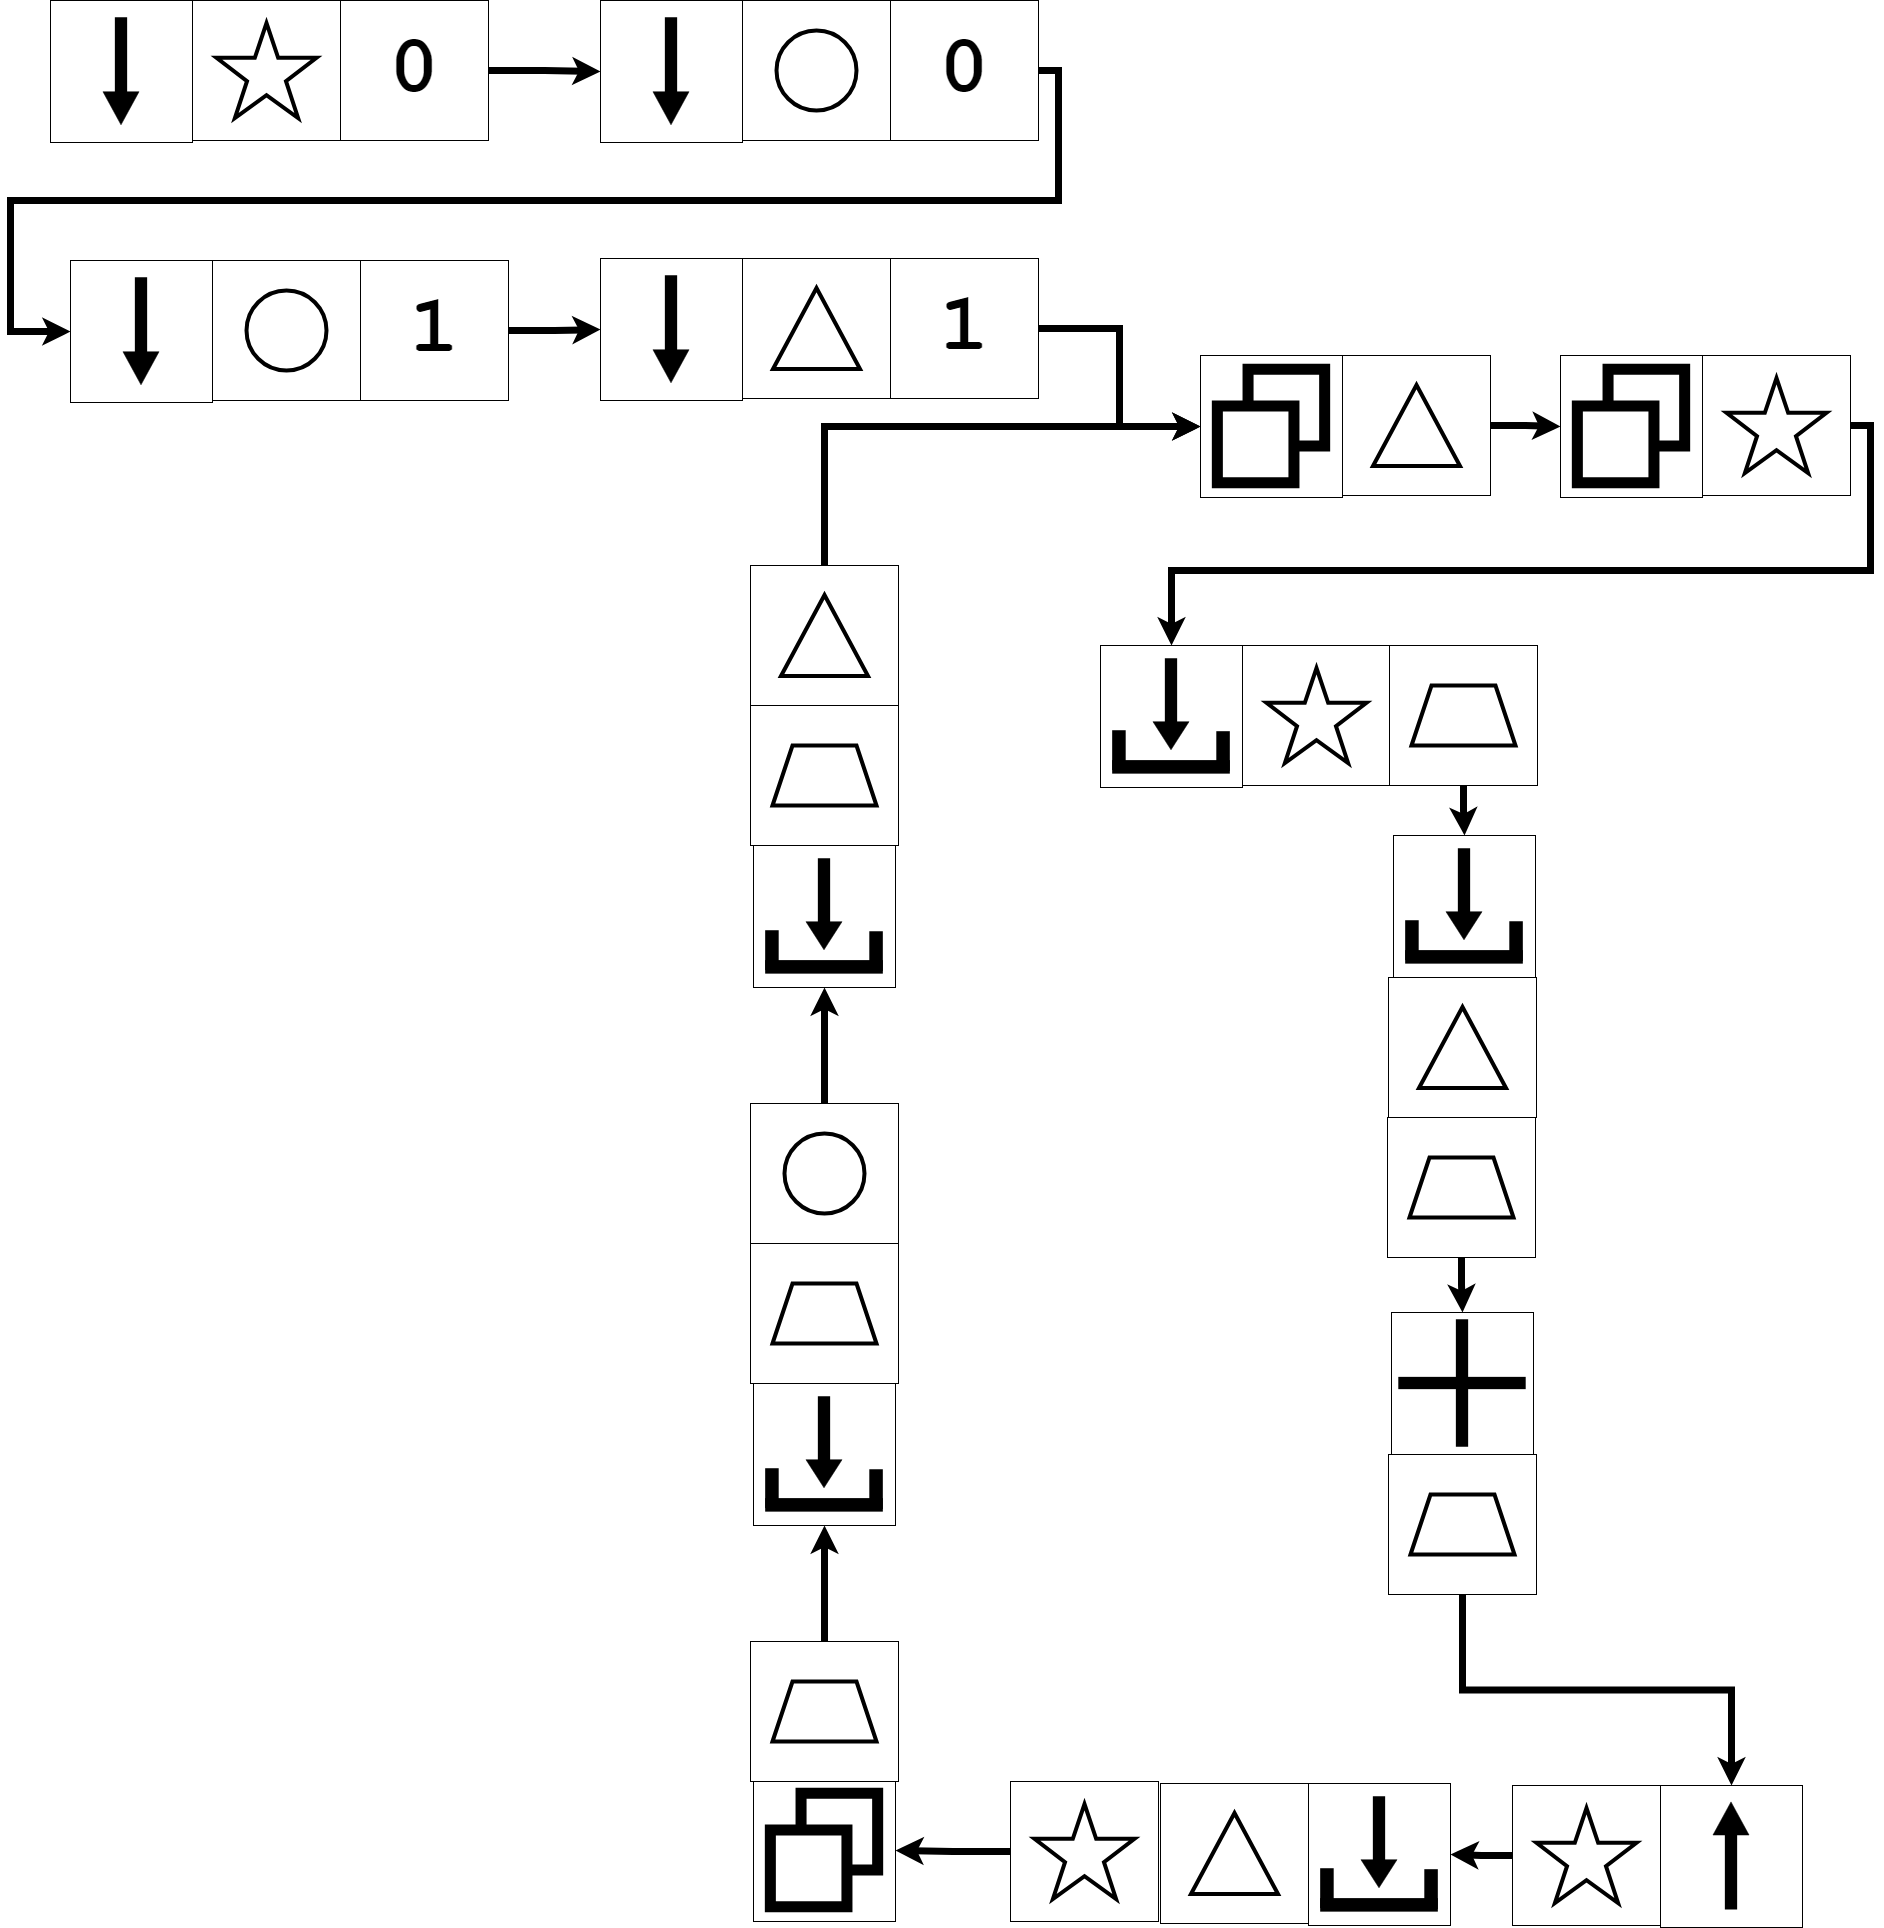
\includegraphics[width=0.5\textwidth]{figures/ArtlangFibpng}
    \caption{\sculpt Fibonacci program}
    \label{fig:artlangfib}
    \vspace{5pt}
\end{figure}

The program in Figure \ref{fig:artlangfib} fills the cirle stack with the numbers of the Fibonacci sequence.

The second notation is a more traditional notation, which is used by the \sculpter interpreter, which will be explained afterwards.
The program is written in a more traditional way, every block has a reserved name, connections are omitted. It reads as a list of instructions, somewhat similar to an assembly language.
Limitations of this implementation are that the program is not visually represented, connections between blocks are not shown and physical loops cannot be represented, forcing the user to only use jump operations for execution control.
Our Fibonacci implementation can be rewritten in \sculpter as follows.

\begin{algorithm}
    \caption{Fibonacci sequence in \sculpt}
    \begin{algorithmic}
    \State $push~0$ \textbf{star}
    \State $push~0$ \textbf{circle}
    \State $push~1$ \textbf{circle}
    \State $push~1$ \textbf{triangle}
    \While{True}
        \State $dup$ \textbf{triangle}
        \State $dup$ \textbf{star}
        \State $mov$ \textbf{star} \textbf{trapezoid}
        \State $mov$ \textbf{triangle} \textbf{trapezoid}
        \State $add$ \textbf{trapezoid}
        \State $pop$ \textbf{star}
        \State $mov$ \textbf{triangle} \textbf{star}
        \State $dup$ \textbf{trapezoid}
        \State $mov$ \textbf{trapezoid} \textbf{circle}
        \State $mov$ \textbf{trapezoid} \textbf{triangle}
    \EndWhile
    \end{algorithmic}
    \end{algorithm}
\endinput

Writing a Fibonacci program is a simple task in \sculpt, yet it is not a complete proof of the language's capabilities.
The language is Turing complete, and it is capable of writing any program that can be written in any other programming language.
To validate this, we will simulate Turing machine in \sculpt.
The Turing machine is a theoretical model of computation that can simulate any algorithm.
For this instance, an implementation od a 3-State Busy Beaver Turing machine will be used.
The Busy Beaver is a theoretical Turing machine that is designed to run for the longest possible time before halting.
Its \sculpt implementation is shown in Figure \ref{fig:busybeaver}.

\begin{figure}
    \centering
    \includegraphics[width=0.5\textwidth]{figures/ArtlangBusyBeaver.png}
    \caption{3-State Busy Beaver Turing machine in \sculpt}
    \label{fig:busybeaver}
    \vspace{5pt}
\end{figure}

Its \sculpter implementation is as follows:

\verbatim{Code still to be added, currently in progress}
